\documentclass[11pt,a4paper]{article}

% Compilar com xelatex (ou lualatex), 2x:
%   xelatex -interaction=nonstopmode relatorio_final.tex
\usepackage{fontspec}
\setmainfont{TeX Gyre Heros}
\setsansfont{TeX Gyre Heros}
\usepackage[brazil]{babel}
\usepackage[a4paper,margin=2.5cm]{geometry}
\usepackage{graphicx}
\usepackage[table]{xcolor}
\usepackage{listings}
\usepackage{booktabs}
\usepackage{array}
\usepackage{tikz}
\usetikzlibrary{positioning,arrows.meta,calc,fit}
\usepackage{fancyhdr}
\usepackage[hidelinks]{hyperref}
\usepackage{enumitem}

\definecolor{corFundo}{RGB}{248,248,248}
\definecolor{corComent}{RGB}{106,115,125}
\definecolor{corKw}{RGB}{167,29,93}
\definecolor{corStr}{RGB}{3,47,98}
\definecolor{corMoldura}{RGB}{210,210,210}
\definecolor{corOk}{RGB}{22,120,50}
\definecolor{corAtk}{RGB}{176,0,32}

\lstset{
  basicstyle=\ttfamily\footnotesize,
  backgroundcolor=\color{corFundo},
  frame=single, rulecolor=\color{corMoldura},
  breaklines=true, columns=fullflexible, keepspaces=true,
  showstringspaces=false, extendedchars=true,
  commentstyle=\color{corComent}\itshape,
  keywordstyle=\color{corKw}\bfseries,
  stringstyle=\color{corStr},
  numbers=left, numberstyle=\tiny\color{corComent}, numbersep=8pt,
  tabsize=4, captionpos=b, xleftmargin=16pt,
}
\lstdefinestyle{saida}{
  language=, keywordstyle=\color{black}, commentstyle=\color{black},
  stringstyle=\color{black}, numbers=none, basicstyle=\ttfamily\scriptsize,
}

\pagestyle{fancy}
\fancyhf{}
\lhead{\small Laboratório de Redes — Relatório Final}
\rhead{\small Interceptação e Defesa}
\cfoot{\thepage}
\renewcommand{\headrulewidth}{0.4pt}

\setlength{\parskip}{0.5em}
\setlength{\parindent}{0pt}

\newcommand{\seta}{\texorpdfstring{$\rightarrow$}{->}}

\begin{document}

% =============================== CAPA ===============================
\begin{titlepage}
\centering
\vspace*{1.5cm}
{\large Pontifícia Universidade Católica do Rio Grande do Sul}\\[0.2cm]
{\large Escola Politécnica}\\[0.2cm]
{\large Laboratório de Redes de Computadores}\\[2.5cm]

\rule{\linewidth}{0.5mm}\\[0.5cm]
{\huge \bfseries Interceptação e Defesa de um\\ Protocolo de Aplicação}\\[0.4cm]
{\Large Relatório Final Consolidado — Fases 1, 2 e 3}\\[0.3cm]
{\large Escuta passiva, MITM ativo e defesa com TLS + autenticação}\\
\rule{\linewidth}{0.5mm}\\[1.5cm]

{\large\bfseries Grupo}\\[0.3cm]
{\large
Gabriel Dienstmann Sieczkowski\\
Lorenzo Hubner Panato\\
Luis Felipe Kvieczinski\\
}
\vfill
{\large Entrega 3 — Defesa e detecção (relatório final das três fases)}\\[0.3cm]
{\large Novembro de 2026}
\end{titlepage}

\tableofcontents
\newpage

% =============================== 1. INTRODUÇÃO ===============================
\section{Objetivo e visão geral das três fases}

Este trabalho demonstra, na prática e em ambiente isolado, por que protocolos de
aplicação sem proteção são vulneráveis — e como uma defesa adequada os
neutraliza. Partiu-se de um serviço-alvo \textbf{propositalmente inseguro}
(autenticação em texto claro) e percorreu-se um arco de três fases:

\begin{itemize}[leftmargin=1.4em]
  \item \textbf{Fase 1 — Escuta passiva.} Um \textit{sniffer} com socket raw lê
  as credenciais que trafegam em texto claro. Demonstra a quebra de
  \textbf{confidencialidade}.
  \item \textbf{Fase 2 — Interceptação ativa (MITM).} Um \textit{proxy}
  man-in-the-middle se posiciona entre cliente e servidor, lê e \textbf{altera}
  mensagens, atendendo várias sessões. Demonstra a quebra de \textbf{integridade
  e autenticação}.
  \item \textbf{Fase 3 — Defesa e detecção.} O canal passa a usar \textbf{TLS}
  com \textbf{certificado} no servidor e \textbf{senhas com hash}. Os ataques das
  fases anteriores deixam de funcionar, e a tentativa de MITM é \textbf{detectada}.
\end{itemize}

O ponto central é que \textbf{o serviço-alvo é o mesmo nas três fases}: o
protocolo de aplicação não muda; mudam o transporte (TCP em texto claro
\seta{} TLS) e o armazenamento de senha (texto claro \seta{} hash). Isso permite
comparar diretamente o ``antes'' e o ``depois''.

% =============================== 2. AMBIENTE ===============================
\section{Ambiente de testes}
\label{sec:ambiente}

Toda a comunicação e a interceptação usam \textbf{sockets diretamente} (sem
frameworks que escondam o socket), em Python 3, usando apenas a biblioteca
padrão (inclusive a camada \texttt{ssl} da Fase 3). Os três hosts do enunciado
(cliente, servidor e observador/atacante) foram isolados com \textbf{network
namespaces do Linux} ligados por uma \textit{bridge}, formando uma rede interna
\texttt{10.0.0.0/24} sem saída para a Internet:

\begin{center}
\begin{tikzpicture}[font=\small,
  host/.style={draw,rounded corners,align=center,minimum width=2.7cm,minimum height=1.1cm},
  atk/.style={host,fill=corAtk!8}]
  \node[host] (cli) {\textbf{cliente}\\\texttt{10.0.0.10}};
  \node[atk,right=2.4cm of cli] (atk) {\textbf{atacante}\\\texttt{10.0.0.30}};
  \node[host,right=2.4cm of atk] (srv) {\textbf{servidor}\\\texttt{10.0.0.20}};
  \draw[-{Latex}] (cli) -- (atk);
  \draw[-{Latex}] (atk) -- (srv);
  \node[below=0.15cm of atk,font=\scriptsize] {bridge \texttt{br-lab} (rede isolada)};
\end{tikzpicture}
\end{center}

Cada host tem IP próprio e o tráfego atravessa a bridge (não a interface de
\textit{loopback}), de modo que a captura reflete uma rede real com três
estações — equivalente, para efeito de observação do tráfego, a três VMs em uma
rede isolada. Os endereços \texttt{10.0.0.10/20/30} que aparecem nas capturas e
logs deste relatório correspondem exatamente a essa topologia. Os scripts
\texttt{demo\_topologia.sh} (Fase 1), \texttt{fase2/demo\_mitm.sh} (Fase 2) e
\texttt{fase3/demo\_defesa.sh} (Fase 3) montam o ambiente e reproduzem os
experimentos automaticamente.

% =============================== 3. FASE 1 ===============================
\section{Fase 1 — Escuta passiva (confidencialidade)}

\subsection{O serviço-alvo}
O protocolo é textual, uma mensagem por linha terminada em \texttt{\textbackslash n},
sobre TCP (porta 5050):

\begin{center}\small
\begin{tabular}{@{}lll@{}}
\toprule
Sentido & Mensagem & Significado \\
\midrule
S \seta{} C & \texttt{200 AUTH-SERVICE v1 pronto} & banner ao conectar \\
C \seta{} S & \texttt{LOGIN <usuario> <senha>} & tentativa de login \\
S \seta{} C & \texttt{200 OK bem-vindo <usuario>} & credenciais válidas \\
S \seta{} C & \texttt{401 ERRO credenciais invalidas} & credenciais inválidas \\
C \seta{} S & \texttt{QUIT} \;/\; S \seta{} C \texttt{221 tchau} & encerramento \\
\bottomrule
\end{tabular}
\end{center}

O servidor (\texttt{servidor.py}) atende cada cliente em uma \textit{thread} e,
na Fase 1, compara a senha recebida diretamente com a base em texto claro
(\texttt{usuarios.txt}). O cliente (\texttt{cliente.py}) envia a credencial sem
qualquer cifragem.

\subsection{O interceptador passivo}
O \texttt{sniffer.py} usa um \textbf{socket raw} (\texttt{AF\_PACKET}/\texttt{ETH\_P\_ALL})
em modo promíscuo: recebe os quadros crus da rede e \textbf{decodifica
manualmente} os cabeçalhos Ethernet, IPv4 e TCP (sem bibliotecas de captura).
Filtrando a porta 5050, ele localiza as linhas \texttt{LOGIN} no payload e exibe
usuário e senha. Também grava um \texttt{.pcap} (formato libpcap escrito à mão)
para conferência no Wireshark.

\subsection{Evidência}
Na captura em texto claro, a credencial aparece legível byte a byte. A metade
superior da Figura~\ref{fig:antesdepois} (coluna ASCII do Wireshark) mostra o
pacote com \texttt{LOGIN alice S3nh4Secreta} — qualquer observador no segmento lê
a senha sem participar da conexão. \textbf{Confidencialidade quebrada.}

% =============================== 4. FASE 2 ===============================
\section{Fase 2 — Interceptação ativa / MITM (integridade e autenticação)}

A Fase 2 adiciona o \texttt{fase2/proxy\_mitm.py}, um intermediário que
\textbf{termina a conexão do cliente e abre outra para o servidor}, repassando as
mensagens nos dois sentidos e podendo \textbf{alterá-las}. O desvio do tráfego é
feito \textbf{por configuração} (o cliente é apontado ao proxy), não por ARP
spoofing. Três adulterações foram implementadas:

\begin{center}\small
\begin{tabular}{@{}lll@{}}
\toprule
Flag & Sentido & Efeito \\
\midrule
\texttt{-{}-forjar-ok} & S \seta{} C & reescreve \texttt{401 ERRO} como \texttt{200 OK bem-vindo} \\
\texttt{-{}-trocar-senha} & C \seta{} S & injeta outra senha na linha \texttt{LOGIN} \\
\texttt{-{}-trocar-usuario} & C \seta{} S & troca o usuário na linha \texttt{LOGIN} \\
\bottomrule
\end{tabular}
\end{center}

No cenário principal (\texttt{-{}-forjar-ok}), o cliente envia uma senha errada; o
servidor \textbf{rejeita} (\texttt{401}); mas o proxy entrega \texttt{200 OK} ao
cliente, que \textbf{aceita como legítimo}. A divergência entre o log do servidor
(\texttt{LOGIN FALHOU}) e o que o cliente recebeu (\texttt{200 OK}) é a prova da
adulteração. O proxy é \textbf{concorrente} (uma \textit{thread} por sentido de
cada sessão, com travas mínimas e justificadas) e \textbf{robusto} (uma sessão
com erro não derruba as demais). \textbf{Integridade e autenticação quebradas.}

% =============================== 5. FASE 3 ===============================
\section{Fase 3 — Defesa e detecção}

A defesa aplica três mecanismos ao \emph{mesmo} serviço, cada um fechando um
vetor explorado antes.

\subsection{Confidencialidade e integridade: TLS}
O \texttt{servidor\_tls.py} envolve o socket TCP em \texttt{ssl.PROTOCOL\_TLS\_SERVER}
e o \texttt{cliente\_tls.py} em \texttt{ssl.PROTOCOL\_TLS\_CLIENT} (TLS~$\geq$~1.2;
na prática o handshake negociou TLS~1.3). A partir daí todo o conteúdo trafega
cifrado e autenticado pelo TLS: um observador vê apenas registros
\texttt{Application Data}, e qualquer alteração de bytes em trânsito quebra a
verificação de integridade do TLS, encerrando a conexão.

\subsection{Autenticação do servidor: certificado}
Foi criada uma \textbf{CA} própria do laboratório (\texttt{gerar\_certificados.sh}).
O servidor apresenta um certificado assinado por essa CA, com o nome lógico
\texttt{servidor-auth} no campo SAN. O cliente confia \textbf{apenas} nessa CA,
exige certificado (\texttt{CERT\_REQUIRED}) e verifica o nome
(\texttt{check\_hostname}). Assim, um MITM que tente se passar pelo servidor
precisa apresentar um certificado válido para \texttt{servidor-auth} assinado
pela CA — o que ele não possui.

\subsection{Autenticação do usuário: senhas com hash}
A base passou de texto claro para \texttt{usuarios\_hash.txt}, com
\textbf{PBKDF2-HMAC-SHA256} e \textbf{salt} aleatório por usuário
(\texttt{gerar\_hashes.py}). O servidor recalcula o hash da senha recebida e
compara em tempo constante (\texttt{hmac.compare\_digest}). As senhas não são mais
armazenadas nem recuperáveis em texto claro.

\subsection{Demonstração: os ataques das Fases 1 e 2 falham}

\paragraph{(a) Antes × depois (o sniffer deixa de ler).}
A Figura~\ref{fig:antesdepois} compara, no mesmo ambiente, o login em texto claro
(Fases 1--2) e com TLS (Fase 3). Em cima, a senha é legível na coluna ASCII do
Wireshark. Embaixo, a captura com TLS só contém \texttt{Client Hello},
\texttt{Server Hello} e \texttt{Application Data} cifrada — uma busca pela string
\texttt{LOGIN} ou pela senha na captura retorna \textbf{zero} resultados. O
\texttt{sniffer.py} da Fase 1, rodado contra o tráfego TLS, captura pacotes mas
\textbf{não extrai nenhuma credencial} (nenhuma linha \texttt{LOGIN} aparece no
payload cifrado).

\begin{figure}[ht]
\centering
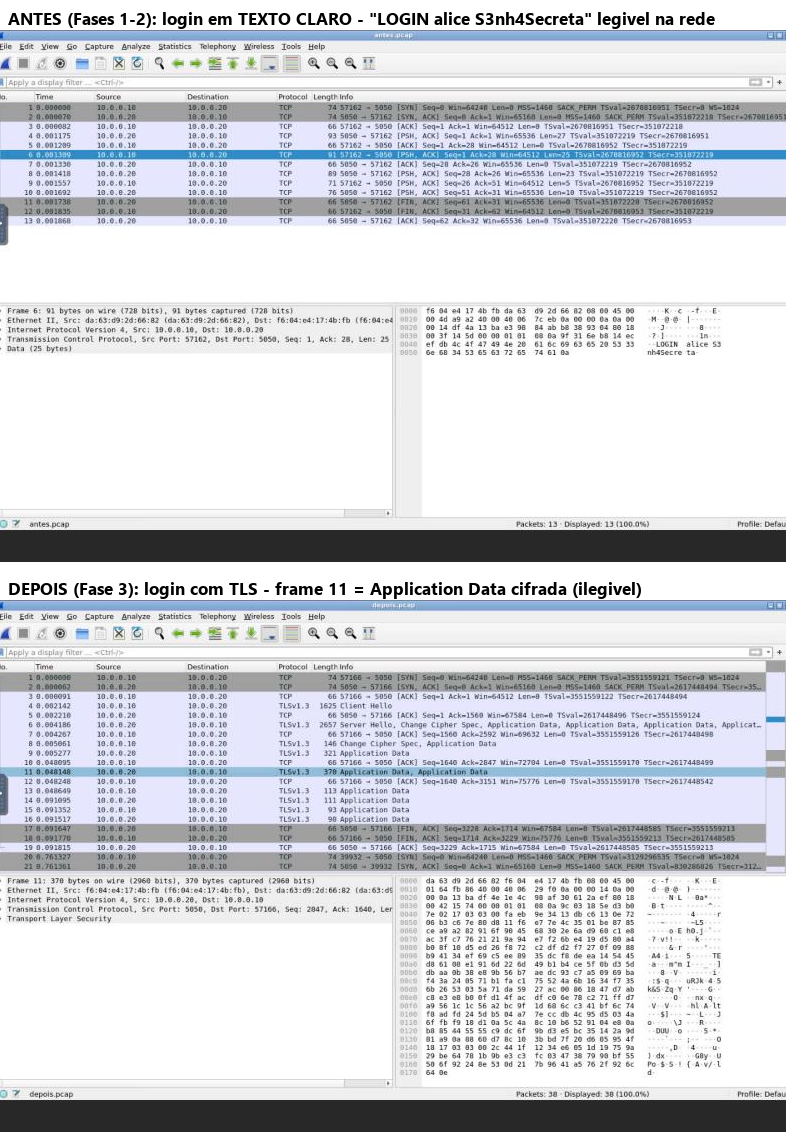
\includegraphics[width=\linewidth,keepaspectratio]{results/fase3/wireshark_antes_depois.png}
\caption{Antes (texto claro, Fases 1--2) × depois (TLS, Fase 3). Em cima, o
Wireshark mostra \texttt{LOGIN alice S3nh4Secreta} legível. Embaixo, o mesmo
login sob TLS: apenas \texttt{Application Data} cifrada, ilegível.}
\label{fig:antesdepois}
\end{figure}

\paragraph{(b) O proxy da Fase 2 não consegue mais adulterar, e o MITM é detectado.}
O \texttt{fase2/proxy\_mitm.py}, que repassa o protocolo linha a linha, só vê
agora bytes cifrados: ele não encontra nenhuma linha \texttt{401} para reescrever
(zero adulterações) e, ao mexer num fluxo que não entende, quebra a sessão TLS.
Para ainda tentar ler ou alterar, o atacante precisaria terminar o TLS se
passando pelo servidor. Apontando o cliente ao atacante
(\texttt{mitm\_tls\_intercept.py}), este tenta
terminar o TLS apresentando um certificado \textbf{auto-assinado}. O cliente
valida contra a CA, vê que o certificado não é confiável e \textbf{aborta antes
de enviar a senha}, com \texttt{CERTIFICATE\_VERIFY\_FAILED}. Na rede
(Figura~\ref{fig:mitm}), isso aparece como um \texttt{Alert (Level: Fatal,
Description: Unknown CA)} enviado pelo cliente, seguido do encerramento da
conexão. Esse alerta é, ao mesmo tempo, a defesa e o \textbf{sinal de detecção}.

\begin{figure}[ht]
\centering
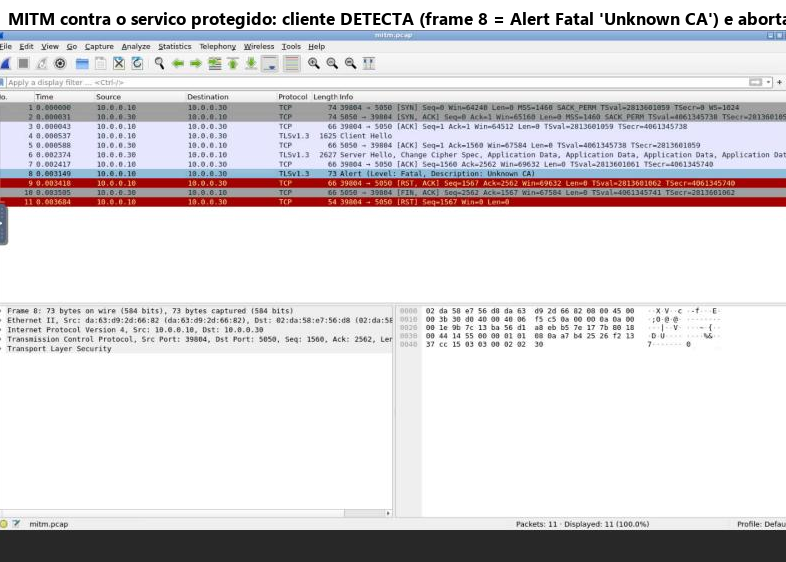
\includegraphics[width=\linewidth,keepaspectratio]{results/fase3/wireshark_mitm_detectado.png}
\caption{MITM contra o serviço protegido. O cliente recusa o certificado do
atacante e emite um \texttt{Alert: Unknown CA} (frame~8), abortando a conexão. A
credencial nunca é enviada.}
\label{fig:mitm}
\end{figure}

Os logs confirmam os dois lados:
\begin{lstlisting}[style=saida]
# CLIENTE
 ATAQUE DETECTADO / CONEXAO ABORTADA
 A validacao do certificado do servidor FALHOU:
   [SSL: CERTIFICATE_VERIFY_FAILED] certificate verify failed: self-signed certificate
 O cliente NAO enviou a credencial.
# ATACANTE
 handshake FALHOU: o cliente recusou o certificado de atacante.
 detalhe TLS: [SSL: TLSV1_ALERT_UNKNOWN_CA] tlsv1 alert unknown ca
 >>> ATAQUE NEUTRALIZADO: a credencial NAO foi enviada.
\end{lstlisting}

% =============================== 6. AMEAÇAS / DETECÇÃO ===============================
\section{Análise de ameaças e detecção}
\label{sec:ameacas}

\begin{center}\small
\renewcommand{\arraystretch}{1.25}
\begin{tabular}{@{}p{3.1cm}p{5.0cm}p{6.0cm}@{}}
\toprule
\textbf{Ameaça} & \textbf{Como a defesa mitiga} & \textbf{Como o defensor detecta} \\
\midrule
Sniffing (leitura passiva) &
TLS cifra todo o conteúdo; o payload vira \texttt{Application Data} &
Não há adulteração a detectar; o próprio cliente confirma a cifra negociada
(\texttt{cipher}) no handshake. \\
MITM / personificação do servidor &
O cliente valida o certificado contra a CA e o nome (SAN) &
Erro \texttt{CERTIFICATE\_VERIFY\_FAILED} no cliente; \texttt{Alert: Unknown CA}
visível na captura; log de \textit{handshake} falho. \\
Adulteração de mensagens &
Integridade do registro TLS (AEAD): alterar bytes quebra a verificação &
Erro de TLS / \texttt{Bad record MAC} e queda da conexão; a sessão não completa. \\
Leitura de senhas no servidor &
PBKDF2 + salt: o arquivo não contém senhas recuperáveis &
Vazamento do arquivo não expõe senhas; tentativas de força bruta ficam caras. \\
Replay (reenvio de tráfego) &
Cada sessão TLS tem chaves e \textit{nonces} próprios; registros reenviados não
decifram &
Falha de decifragem/integridade na nova sessão; a sessão antiga não é reutilizável. \\
\bottomrule
\end{tabular}
\end{center}

Em resumo, a detecção de um ataque ativo é \textbf{explícita e local ao cliente}:
a validação do certificado falha \emph{antes} de qualquer dado sensível ser
enviado, e o evento é observável tanto no log da aplicação quanto na captura de
rede (o alerta TLS).

% =============================== 7. LIMITAÇÕES ===============================
\section{Limitações da defesa}

\begin{itemize}[leftmargin=1.4em]
  \item \textbf{Metadados continuam visíveis.} TLS cifra o conteúdo, mas não os
  IPs, portas, tamanhos e tempos dos pacotes. Um observador ainda sabe
  \emph{quem} fala com \emph{quem}, \emph{quando} e \emph{quanto}.
  \item \textbf{Confiança na CA.} A segurança depende de o cliente confiar apenas
  na CA correta. Se um atacante conseguir inserir sua CA na lista de confiança do
  cliente (ou comprometer a CA), a personificação volta a ser possível.
  \item \textbf{Apenas o servidor é autenticado por certificado.} O cliente é
  autenticado só pela senha (sobre o canal seguro). Autenticação mútua (mTLS,
  com certificado também no cliente) seria uma extensão natural.
  \item \textbf{Comprometimento de endpoint.} TLS protege o canal, não as pontas.
  Se o cliente ou o servidor for comprometido, o conteúdo é exposto na origem.
  \item \textbf{Fora de escopo.} Ataques de negação de serviço, exploração de
  vulnerabilidades da implementação de TLS e engenharia social não são tratados.
\end{itemize}

% =============================== 8. CONCLUSÃO ===============================
\section{Conclusão}

As três fases, sobre o mesmo serviço, mostram o ciclo completo de uma falha de
segurança de transporte e sua correção. Sem proteção, um observador \textbf{lê}
as credenciais (Fase 1) e um intermediário \textbf{mente} para os dois lados
(Fase 2) sem ser percebido. Com TLS, certificado no servidor e senhas com hash
(Fase 3), o mesmo sniffer passa a ver apenas bytes cifrados, o mesmo MITM é
\textbf{detectado e recusado} antes de obter qualquer credencial, e as senhas
deixam de existir em texto claro. A defesa não é absoluta — metadados, confiança
na CA e comprometimento de endpoint permanecem como limites — mas elimina
exatamente as ameaças de confidencialidade, integridade e autenticação que as
Fases 1 e 2 demonstraram.

\end{document}
